\setchapterpreamble[u]{\margintoc}
\chapter{Energy History}
\labch{energy_history}

In this chapter I go over human history with energies, and how energy is a limiting factor. We also go over a 100\% renewable world, the past.


By taking high resolution satellite imagery of the Earth at Night, and combining this with high resolution population data, we can estimate the regions of the world in energy poverty. \vreffig{energy_poverty} shows where energy poverty exist.

We still have a long way to go\ldots

\begin{figure*}[h]
	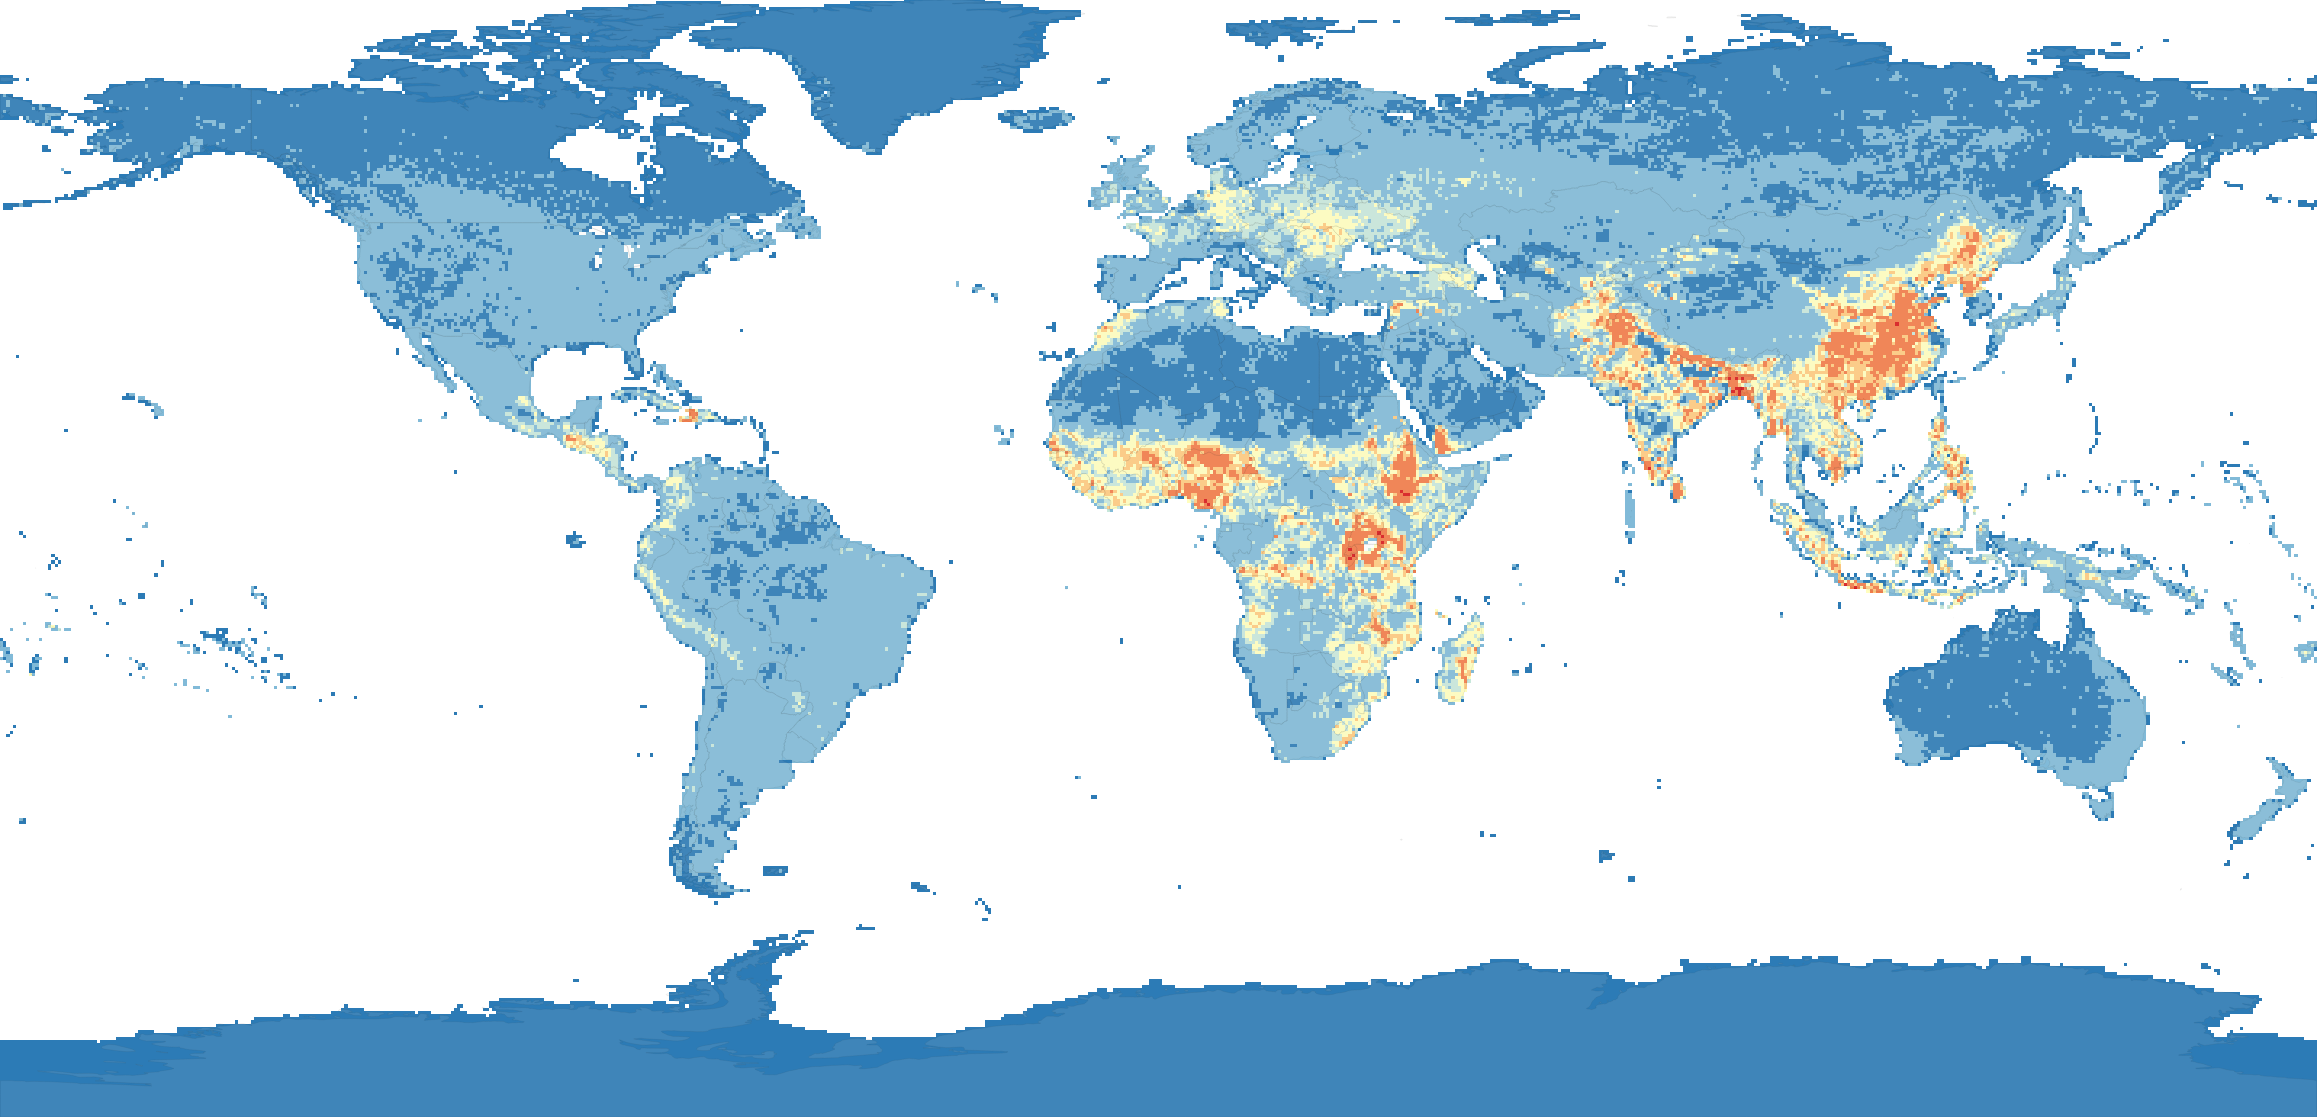
\includegraphics[width=1.0\textwidth]{energy_poverty_05deg_3mwh_cf95}
	\caption[Energy poverty in the world.]{Energy poverty in the world.}
	\labfig{energy_poverty_world}
\end{figure*}


\section{The Digest}

\begin{kaoboxgreen}[frametitle=Main Takeaways]

\begin{itemize}
\item This has not been done yet
\item Reading this will teach you absolutely nothing
\item I am serious, I could type random letters and it would give you as much information
\item Fedhiz gavartz hedtz inewps
\end{itemize}
  
\end{kaoboxgreen}